\documentclass[10pt,a4paper]{article}
\usepackage[latin1]{inputenc}
\usepackage[dutch]{babel}
\usepackage{amsmath}
\usepackage{amsfonts}
\usepackage{amssymb}
\usepackage{graphicx}
\usepackage{listings}
\author{Ruben Van Assche - S0122623}
\title{Wetenschappelijk Programmeren: Data Smoothing - Oefening 5}
\begin{document}
\maketitle
\section{Opgave}
In deze opgave moest voor $n = 6, 7, 8, 11, 13, 15$ een veelterm worden bepaald d.m.v. de kleinste kwadraten methode die de 17 punten tussen [-1, 1] benadert van de Runge functie.

\section{Opstellen van het model}
Bij Data Smoothing gaan we proberen het residu te minimaliseren. Dit betekent dus dat we volgende vergelijkingen willen minimaliseren:
$$ \sum_{i = 1}^{m} \left [ y_{i} - \sum_{j = 1}^{n} a_{ij} \lambda_{j}  \right ]^{2} $$
Hierbij is $y_{i}$ een vector met de y-Waarden van de Runghe functie. Deze kunnen makkelijk worden berekend uit de opgave: 0.03846, 0.04965, 0.06639, 0.09289, 0.1379, 0.2215, 0.3902, 0.7191, 1, 0.7191, 0.3902, 0.2215, 0.1379, 0.09289, 0.06639, 0.04965, 0.03846.
\newline
\newline
De bijhorende x-waarden zijn: -1, -0.875, -0.75, -0.625, -0.5, -0.375, -0.25, -0.125, 0, 0.125, 0.25, 0.375, 0.5, 0.625, 0.75, 0.875, 1.
\newline
\newline
De A matrix waaruit we $a_{ij}$ halen is een $m x n+1$ matrix waarbij op elke rij een x waarde tot een bepaalde macht wordt verhoffen. Deze macht wordt bepaald door de kolom waar deze x waarde in staat. Staat de waarde bijvoorbeeld in de 3de kolom dan wordt deze tot de tweede macht verhoffen. Staat deze in de 4de kolom dan wordt deze tot de 3de macht verhoffen enzovoorts.
\newline
\newline
De matrix A ziet er dan als volgt uit:
$$
\begin{bmatrix}
x_{1}^{0} & x_{1}^{1}  & \cdots  & x_{1}^{n} \\ 
x_{2}^{0} &x_{2}^{1}   & \cdots  & x_{2}^{n} \\ 
\vdots  &\vdots   &  & \vdots  \\ 
x_{m}^{0} & x_{m}^{1}  & \cdots  & x_{m}^{n} 
\end{bmatrix}
$$
De $\lambda$ vector is op deze moment onbekend maar heeft een grootte van n + 1.

\section{Berekenen van de lambda vector}
De factoren in de lambda vector worden berekend met een lineaire multiparameter regressie. GSL voorziet hiervoor een functie $\textit{gsl multifit linear}$. Aan deze functie worden de A matrix, y vector en $\lambda$ vector meegegeven. GSL berekent dan de waarden in de $\lambda$ vector d.m.v. singular value decomposition van de matrix A  gebruikmakend  van het gewijzigde Golub-Reinsch SVD algoritme.
\newline
\newline
De factoren in de $\lambda$ vector zullen uiteindelijk de coefficienten van de veelterm vergelijking vormen die de gegeven punten probeert te benderen.
\newline
\newline
Vervolgens berekenen we d.m.v. $\textit{gsl multifit linear residuals}$ de residu's deze worden bepaald door: $y - A * \lambda$ en zullen later nog gebruikt worden.

\section{De verglijkingen}
Van zodra de factoren in de $\lambda$ vector bepaald zijn kunnen we vergelijkingen voor de veelterm opstellen:
\begin{center}
\textbf{n = 6}
\end{center}
$Y = 0.7689993515  + 9.414854674e-16 X -4.336109672 X^{2}  + 1.281502612e-15 X^{3}  + 7.777329573 X^{4} -1.282551025e-15 X^{5} -4.196381387 X^{6} $
\begin{center}
\textbf{n = 7}
\end{center}
$Y = 0.7689993515  + 2.688093862e-16 X -4.336109672 X^{2} -4.841921829e-16 X^{3}  + 7.777329573 X^{4}  + 1.168264296e-15 X^{5} -4.196381387 X^{6} -1.184527236e-15 X^{7} $
\begin{center}
\textbf{n = 8}
\end{center}
$Y = 0.8501998604 -7.258487361e-15 X -7.161857918 X^{2}  + 1.683022793e-14 X^{3}  + 22.70956181 X^{4} -4.307021306e-15 X^{5} -28.9036082 X^{6} -1.385842305e-14 X^{7}  + 12.54970251 X^{8}  $
\begin{center}
\textbf{n = 11}
\end{center}
$Y = 0.9072324888  + 7.140610879e-14 X -10.37101681 X^{2} -2.101452267e-12 X^{3}  + 50.95571241 X^{4}  + 1.247554915e-11 X^{5} -114.269923 X^{6} -3.017527929e-11 X^{7}  + 116.0762224 X^{8}  + 3.187811671e-11 X^{9} -43.26056639 X^{10} -1.218867951e-11 X^{11} $
\begin{center}
\textbf{n = 13}
\end{center}
$Y = 0.9471737963 -1.584623709e-13 X -13.82653137 X^{2}  + 8.181339107e-12 X^{3}  + 98.4047674 X^{4} -1.02533859e-10 X^{5} -347.9856535 X^{6}  + 4.680857313e-10 X^{7}  + 626.8761862 X^{8} -9.684471789e-10 X^{9} -548.6596796 X^{10}  + 9.222148256e-10 X^{11}  + 184.2822627 X^{12} -3.274590204e-10 X^{13} $
\begin{center}
\textbf{n = 15}
\end{center}
$Y = 0.9754849108  + 1.116712052e-12 X -17.55205188 X^{2}  + 3.664490199e-12 X^{3}  + 176.6106197 X^{4} -5.865735805e-11 X^{5} -949.2311491 X^{6} -2.544832873e-10 X^{7}  + 2775.990946 X^{8}  + 2.826537973e-09 X^{9} -4398.964036 X^{10} -7.514213553e-09 X^{11}  + 3525.205695 X^{12}  + 8.033802204e-09 X^{13} -1112.997048 X^{14} -3.038144153e-09 X^{15} $
\section{De residu's}
De residu's zijn ook berekend, om deze beter te interpreteren heb ik de $\l_{2}$ norm van de vector genomen:
\newline
\begin{center}
\begin{tabular}{ll}
\textbf{N} & \textbf{Residu}         \\
6          & 0.36469983584691223477  \\
7          & 0.3646998358469124013   \\
8          & 0.23782656759792672463  \\
11         & 0.14938135629848825481  \\
13         & 0.08844594204494805878  \\
15         & 0.046700465578771409303
\end{tabular}
\end{center}
\section{Plots}
Hieronder een plot van de originele gegeven punten + voor elke n een verglijking geplot.
\newline
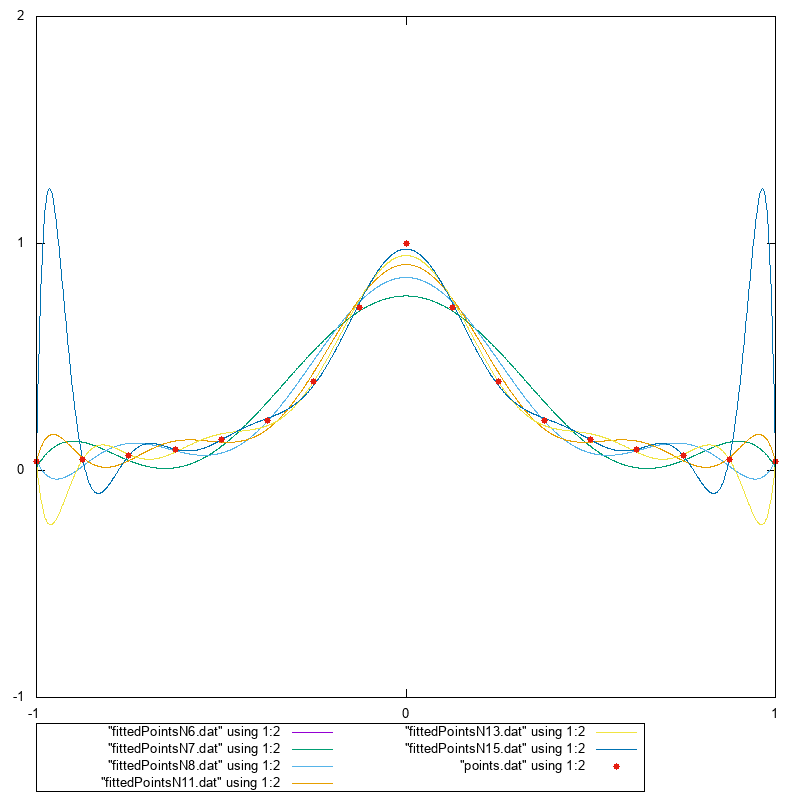
\includegraphics[scale=0.6]{fit}
\section{Bevindingen}
\subsection{Minimale Residu's}
Naarmate n stijgt, worden de residu's kleiner waardoor de veelterm steeds dichter bij de gegeven punten ligt(zie hiervoor ook de plots).
\subsection{Beste plot}
We zien dat de veelterm met een hogere n dichter bij de gegeven punten liggen maar natuurlijk zorgt dit ook weer voor het Runghe fenomeen(zie de uiteindes). Dus dan lijkt een veelterm met een lagere n wel beter. Het wijzigen van basis zou er voor kunnen zorgen dat we toch een veelterm met hogere n kunnen gebruiken met minder last van het Runghe fenomeen.
\subsection{Ontbreken van n = 7}
Dit fenomeen snap ik niet echt: de vergelijkingen gegenereerd uit de $\lambda$ vector zijn dan wel verschillend voor $n = 6$ en $n = 7$ de punten die eruit worden gegenereerd zijn exact hetzelfde. Dit is raar want voor alle andere n komen er andere punten uit. Ik heb ook een als test $n = 5$ berekend(omdat misschien bij lagere n om een of andere reden de punten hetzelfde zijn) maar deze genereert ook verschillende punten t.o.v. $n = 6$ en $n = 7$.
\section{Code}
\textbf{Main.cpp - De code voor alle berekeningen}
\lstinputlisting{../main.cpp}

\end{document}